\documentclass[twoside,11pt]{article}
\usepackage{jmlr2e}
\usepackage{graphicx}
\graphicspath{ {./images/} }
\usepackage{enumitem}
\newlist{mylistenv}{enumerate}{3}
\newenvironment{mylist}[1]{%
	\setlist[mylistenv]{label=#1\arabic{mylistenvi}.,ref=#1\arabic{mylistenvi}}%
	\setlist[mylistenv,2]{label=#1\arabic{mylistenvi}.\arabic{mylistenvii}.,ref=#1\arabic{mylistenvi}.\arabic{mylistenvii}}%
	\setlist[mylistenv,3]{label=#1\arabic{mylistenvi}.\arabic{mylistenvii}.\arabic{mylistenviii}.,ref=#1\arabic{mylistenvi}.\arabic{mylistenvii}.\arabic{mylistenviii}}%
	\renewenvironment{mylist}{\begin{mylistenv}}{\end{mylistenv}}
	\begin{mylistenv}%
	}{%
	\end{mylistenv}%
}

% Definitions of handy macros can go here

\newcommand{\dataset}{{\cal D}}
\newcommand{\fracpartial}[2]{\frac{\partial #1}{\partial  #2}}


\firstpageno{1}

\begin{document}

\title{Project 2: \textit{k} Nearest Neighbors}

\author{\name Sarah Wilson 
	   \email swi1s117@jhu.edu \\
	   \phone 303-921-7225 \\
       \addr Engineering Professionals Computer Science\\
       Johns Hopkins University\\
       Baltimore, MD 21218, USA} 

\maketitle


\section{Introduction}
Regression and classification are both common tasks in the realm of Machine Learning. Regression and classification are both supervised learning problems. Supervised learning is where the system is given an input and output and then asked to learn or predict the mapping of input to output. The algorithm explored in this paper is \textit{k}-Nearest Neighbor (\textit{k}NN). \textit{k}NN is an example of a nonparametric algorithm, nonparametic algorithms do not make any strong assumptions about the form of the mapping function from input data to output predictions. The advantage offered by this approach is that not a lot of prior knowledge on the data or its features is required to build a predictor. \textit{k}NN is nonparametric as it makes predictions for new data based upon training data by looking at the \textit{k} closest neighbors to the new data. The primary philosophy behind the \textit{k}NN algorithm is ""(INSERT REF)\\ 

\hspace*{10mm} INSERT REFERENCES ON APPLICATIONS\\

\hspace*{10mm} The problem statement presented in this paper is to understand and implement a \textit{k}NN classifier and regressor on 6 different and unique data sets. The experimentation will first be tuned using a validation subset of the overall data set under experimentation, to determine the most optimal value of \textit{k} to use. Then the optimal value of \textit{k} will be run through the full \textit{k}-fold cross validation process. The experimentation will examine: \textit{k}NN, edited \textit{k}NN and condensed \textit{k}NN The results presented will be the classification error and the regression mean squared error on each of the 6 unique data sets and across the 3 variations of the  \textit{k}NN algorithm.\\

\hspace*{10mm} The hypothesis of this report is that INSERT\\

\hspace*{10mm} Section 1 has provided the introduction, problem statement and hypothesis in regards to the \textit{k}NN algorithm. Section 2 will provide an in-depth explanation of the \textit{k}NN algorithm, how the algorithm will be tuned and specifics on each of the 6 data sets used. Section 3 will present the results obtained by variations of \textit{k}NN, edited \textit{k}NN and condensed \textit{k}NN and the values that were chosen as part of the tuning process. Section 4 will discuss the results that were obtained and compare them to the hypothesis that was outlined in the introduction. This report will conclude in Section 5 with a discussion of lessons learned and areas of possible future work.\newline



\section{Algorithms and Experimental Methods}
The experimental method used in this report is \textit{k}-Fold Cross Validation. \textit{k}-Fold Cross Validation is used when the data sets that an algorithm is being experimented on is small, the goal of \textit{k}-Fold Cross validation is to maximize the amount of data that is used for training of the algorithm. The expriment will use 5-Fold Cross Validation ($\textit{k} = 5$).\\ 
For the experiment in this report a Validation / Tuning set is first used to determine the optimal value of \textit{k} neighbors in the \textit{k}NN.\\ 

\textbf{General \textit{k}NN}\\
\hspace*{10mm} The approach is outlined in the steps below for the General \textit{k}NN algorithm implementation:

\begin{mylist}{Step }
	\item Load in Entire data set 
	\item Randomly shuffle the Entire data set
	\item \textbf{Start Validation / Tune Process}
	\begin{mylist}
		\item Remove 20\% of data point from Entire data set, assign to new Validation / Tune  data set. 
		
	\end{mylist}
	

\end{mylist}

\textbf{Edited \textit{k}NN}\\
\hspace*{10mm} The approach is outlined in the steps below for the Edited \textit{k}NN algorithm implementation:\\

\textbf{Condensed \textit{k}NN}\\
\hspace*{10mm} The approach is outlined in the steps below for the Condensed \textit{k}NN algorithm implementation:\\


\begin{center}
%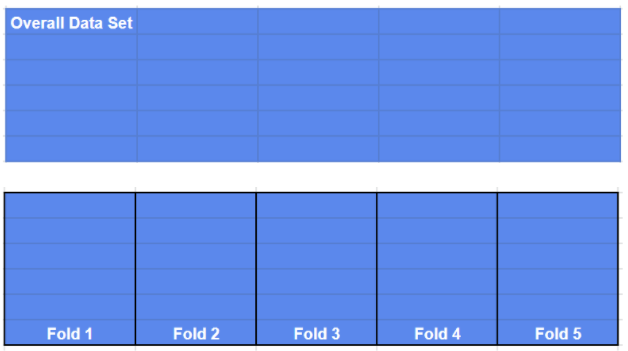
\includegraphics[scale=.6]{kfold1}\newline 
%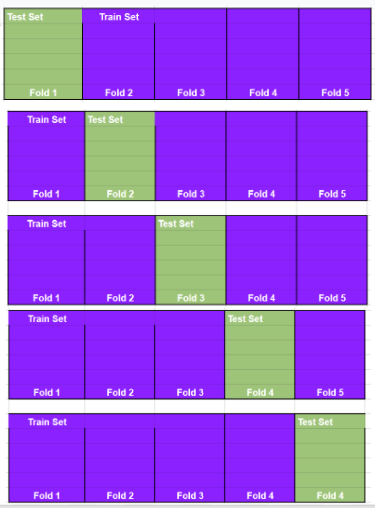
\includegraphics[scale=1]{kfold2}\newline 
\end{center}






\newpage
{\noindent}{\bf Data Sets}\newline
The following data sets were used during the classification and regression tasks for this project.\newline
{\bf Breast Cancer}\newline
Description: \newline
Task: Classification\newline
Predictor: Diagnosis (Malingant or Benign)\newline
Link:\newline \url{https://archive.ics.uci.edu/ml/datasets/Breast+Cancer+Wisconsin+%28Original%29}\newline
{\noindent}\textbf{Car Evaluation}\newline
Description:\newline
Task: Classification\newline
Predictor: Car Evaluation (Unacceptable, Acceptable, Good, Very Good)\newline
Link: \newline
\url{https://archive.ics.uci.edu/ml/datasets/Car+Evaluation}\\
{\noindent}\textbf{Congressional Vote}\newline
Description: 1984 United Stated Congressional Voting Records\newline
Task: Classification \newline
Predictor: Party (Reblican / Democrat) \newline
Link: \newline
\url{https://archive.ics.uci.edu/ml/datasets/Congressional+Voting+Records}\newline
{\noindent}\textbf{Albalone}\newline
Description: Physical merasurements of Albalone\newline
Task: Regression\newline
Predictor: Rings (int)\newline
Link: \newline
\url{https://archive.ics.uci.edu/ml/datasets/Abalone}\newline
{\noindent}\textbf{Computer Hardware}\newline
Description: Realative CPU performance data.\newline
Task: Regression\newline
Predictor: PRP\newline
Link: \newline
\url{https://archive.ics.uci.edu/ml/datasets/Computer+Hardware}\newline
{\noindent}\textbf{Forest Fires}\newline
Description: Forest Fire burn area data\newline
Task: Regression\newline
Predictor: Area (float)\newline
Link: \newline
\url{https://archive.ics.uci.edu/ml/datasets/Forest+Fires}\newline
	
\newpage

\section{Results}
The following results were obtained from the Classification task data sets.
Tables 1-3 display the results from the Breast Cancer, Car Evaluation and Congressional Vote data sets. These tables show the result from the train set and the test set during each fold of the \textit{k}-fold validation process. The tables also display the accuracy and error obtained during each fold, and the total accuracy and error as averaged across each of the 5 \textit{k}-folds. An accuracy(scale of 0-1) of 1 indicates that the train set had the most frequently occurring classifier equal to the most frequently occurring classifier in the test set. An error(scale of 0-1) of 0 indicates that the test set and train set had the same most frequently occurring classifier. Note in the Breast Cancer data set a value of 2 was mapped to the classifier of benign.\\ 

\begin{table}[h!]
	\begin{center}
		\caption{Breast Cancer: Naive Majority Predictor Results}
		\label{tab:table1}
		%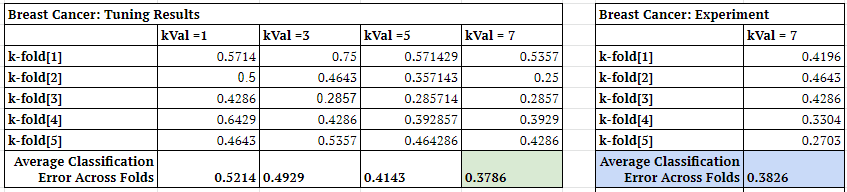
\includegraphics[scale=.6]{BC_Results}\newline
	\end{center}
\end{table}

\begin{table}[h!]
	\begin{center}
		\caption{Car Evaluation: Naive Majority Predictor Results}
		\label{tab:table2}
		%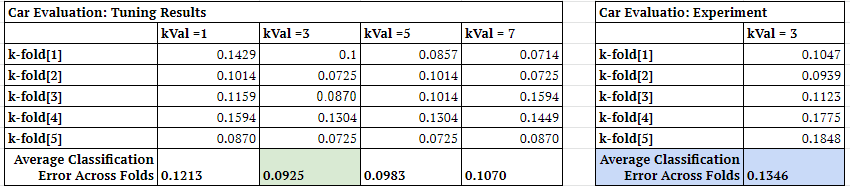
\includegraphics[scale=.6]{CE_Results}\newline
	\end{center}
\end{table}

\begin{table}[h!]
	\begin{center}
		\caption{Congressional Vote: Naive Majority Predictor Results}
		\label{tab:table3}
		%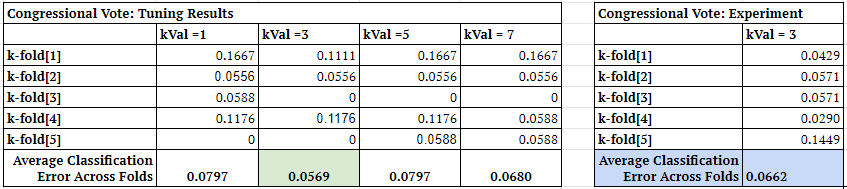
\includegraphics[scale=.6]{CV_Results}\newline
	\end{center}
\end{table}
\newpage

The following results were obtained from the Regression task data sets. Tables 4-6 display the results from the Albalone, Computer Hardware and Forest Fire data sets. These tables show the result from the train set and the test set during each fold of the \textit{k}-fold validation process.  The tables also display the error obtained during each fold, and the total error as averaged across each of the 5 \textit{k}-folds The error is the absolute error and was calculated as: $| Test Set Average - Train Set Average|$. This is meant as a measure of how far off the train set average was from the test set average. 

\begin{table}[h!]
	\begin{center}
		\caption{Albalone: Naive Mean Predictor Results}
		\label{tab:table4}
		%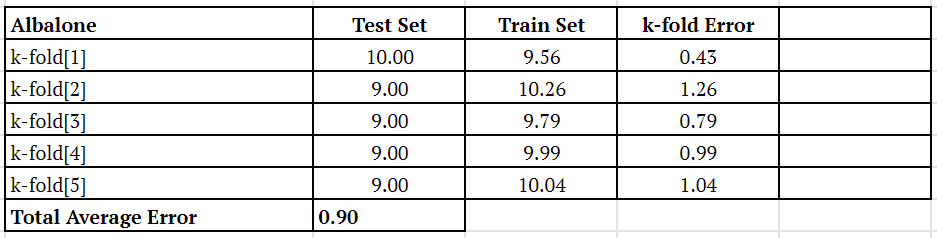
\includegraphics[scale=.6]{AB_Results}\newline
	\end{center}
\end{table}

\begin{table}[h!]
	\begin{center}
		\caption{Computer Hardware: Naive Mean Predictor Results}
		\label{tab:table5}
		%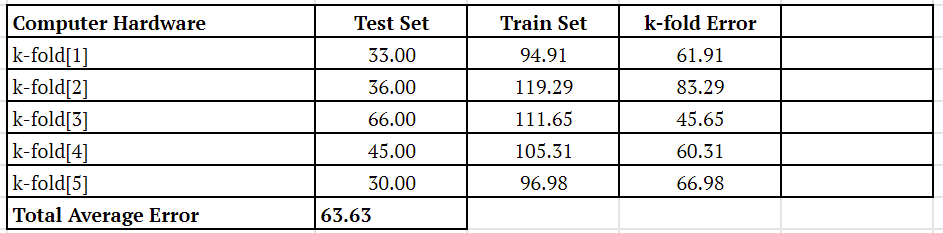
\includegraphics[scale=.6]{CH_Results}\newline
	\end{center}
\end{table}

\begin{table}[h!]
	\begin{center}
		\caption{Forest Fire: Naive Mean Predictor Results}
		\label{tab:table6}
		%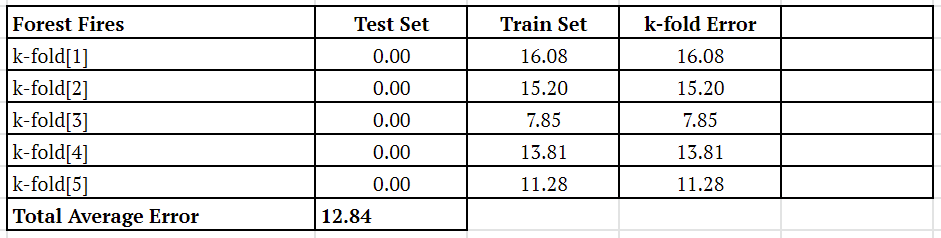
\includegraphics[scale=.6]{FF_Results}\newline
	\end{center}
\end{table}



\newpage

\section{Discussion}
INSERT\\ 

\section{Conclusion}
INSERT\\ 

\newpage


\end{document}